\documentclass{article}
\usepackage[utf8]{inputenc}

% Page setup
\usepackage[a4paper,landscape,margin=2cm]{geometry}
\usepackage{amsmath}

% Typography
\usepackage[scaled]{helvet}
\let\familydefault\sfdefault

\usepackage[usenames,svgnames]{xcolor}
\usepackage{tikz,pgfplots}
\usetikzlibrary{positioning,arrows,intersections,calc,shapes}

\definecolor{one}  {RGB}{142, 23,  4}
\definecolor{two}  {RGB}{ 62,111,186}
\definecolor{three}{RGB}{172,196, 75}
\newcommand\plotfontsize{\fontsize{6}{6}\selectfont}
\pgfplotsset{%
  compat=1.6,
  xmin=0.9, xmax=270,
  axis lines=left,
  every axis/.append style={
    font=\plotfontsize,
  },
  label style={
    font=\plotfontsize\bfseries,
  },
  tick label style={
    font=\plotfontsize,
  },
  legend cell align=left,
  legend style={
    /tikz/every even column/.append style={column sep=.3em},
    draw=none, fill=none,
    inner sep=0pt, outer sep=0pt,
    anchor=north east,
    text height=3pt,
  },
  legend image post style={only marks},
  log base 10 number format code/.code={%
    $\pgfmathparse{10^(#1)}\pgfmathprintnumber{\pgfmathresult}$%
  },
  % Don't show axis exponent
  ytick scale label code/.code={},
}

\begin{document}
\pagestyle{empty}
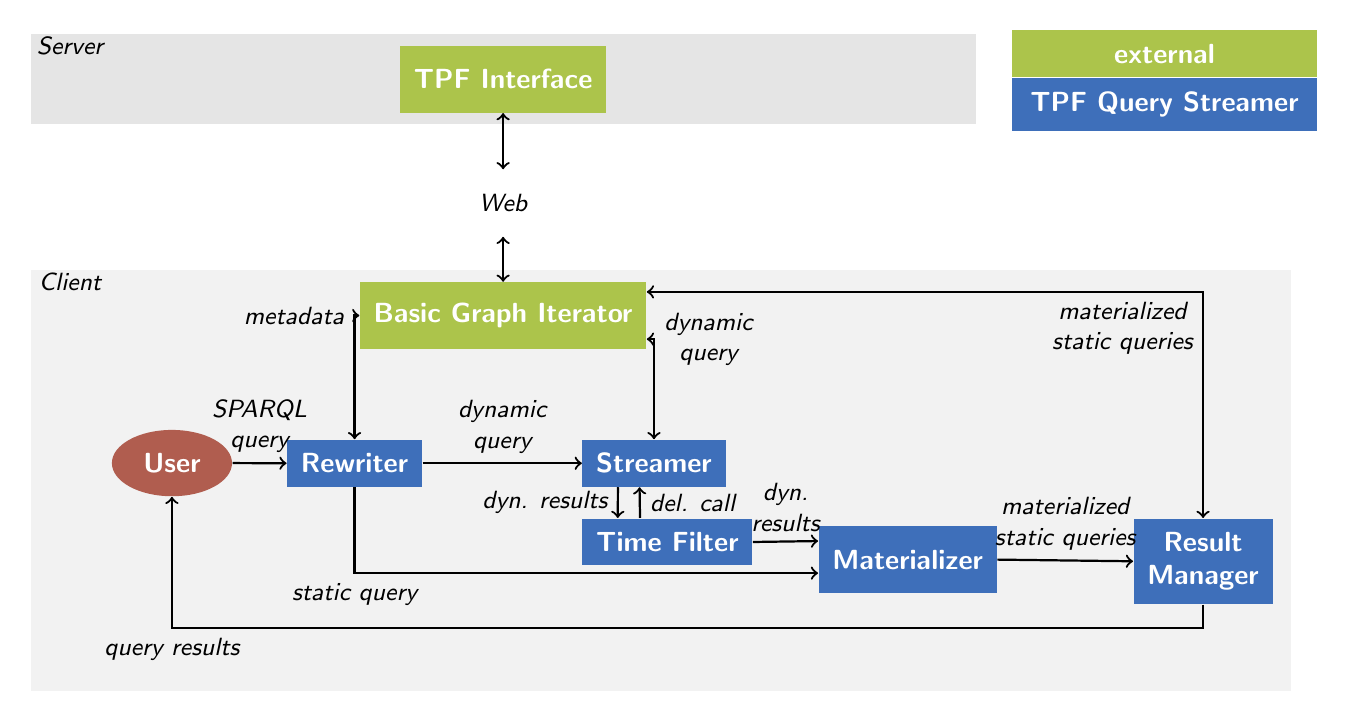
\begin{tikzpicture}[
  font={\sffamily\itshape\small},
  component/.style={fill=three,text=white,font={\sffamily\bfseries},inner sep=5pt,align=center},
  qscomponent/.style={fill=two,text=white,font={\sffamily\bfseries},inner sep=5pt,align=center},
  user/.style={ellipse,fill=one!70,text=white,font={\sffamily\bfseries},inner sep=5pt,align=center},
  tall/.style={minimum height=24pt},
]

  % Make distinction between server/client
  \fill[black!10!white] (2,5.15) rectangle (14,4);
  \fill[black!5!white] (2,2.15) rectangle (18,-3.2);
  \node at(2.5,5) {Server};
  \node at(2.5,2) {Client};
  %\draw[-,thick,xshift=-1] (2,4) -- (18,4) node [above,midway,align=center] {Server};
  %\draw[-,thick,xshift=-1] (2,2.15) -- (18,2.15) node [below,midway,align=center] {Client};
  
  % Legend
  \node[component,text width=100pt] at(16.4,4.9) {\itshape external};
  \node[qscomponent,text width=100pt] at(16.4,4.25) {\itshape TPF Query Streamer};
  
  \node[below right,user] (client) at (3.25,0) {User};
  
  \node[below right,qscomponent] (rewriter) at (5.25,0) {Rewriter};
  
  \node[below right,qscomponent] (streamer) at (9,0) {Streamer};
  
  \node[below right,qscomponent] (filter) at (9,-1) {Time Filter};
  
  \node[below right,qscomponent,tall] (materializer) at (12,-1.1) {Materializer};
  
  \node[below right,qscomponent] (resultmgr) at (16,-1) {Result\\Manager};
  
  \node[below,component,tall] (ldfclient) at (8,2) {Basic Graph Iterator};
  
  \node[inner sep=0pt,tall] (web) at (8,3)
        [align=center] {Web};
  
  \node[below,component,tall] (ldfserver) at (8,5) {TPF Interface};
  
  
  \draw[->,thick] (client.east) -- (rewriter.west) node [above,midway,align=center] {SPARQL\\query};
  
  \draw[<->,thick] (rewriter.north) |- (ldfclient.west) node [left,midway] {metadata};
  
  \draw[->,thick] (rewriter.east) -- (streamer.west) node [above,midway,align=center] {dynamic\\query};
  \draw[->,thick] (rewriter.south) |- ($ (materializer.west)!0.4!(materializer.south west)$) node [below,midway] {static query};
  
  \draw[<->,thick] (streamer.north) |- ($ (ldfclient.east)!0.7!(ldfclient.south east)$) node [right,midway,align=center] {dynamic\\query};
  
  \draw[->,thick] ($ (streamer.south)!0.5!(streamer.south west)$) -- ($ (filter.north)!0.58!(filter.north west)$) node [left,midway] {dyn. results};
  \draw[<-,thick] ($ (streamer.south)!0.2!(streamer.south west)$) -- ($ (filter.north)!0.32!(filter.north west)$) node [right,midway] {del. call};
  \draw[->,thick] (filter.east) -- ($ (materializer.west)!0.55!(materializer.north west)$) node [above,midway,align=center] {dyn.\\results};
  %\draw[->,densely dotted] (filter.south) -- (streamer.south) node {\emph{Delayed call}};
  
  \draw[->,thick] (materializer.east) -- (resultmgr.west) node [above,midway,align=center] {materialized\\static queries};
  
  \draw[<->,thick] (resultmgr.north) |- ($ (ldfclient.east)!0.7!(ldfclient.north east)$) node [below left,midway,align=center] {materialized\\static queries};
  
  \draw[->,thick] (resultmgr.south) -- ++(0,-0.3) -| (client.south) node [below,midway] {query results};
  
  \draw[<->,thick] (ldfclient.north) -- (web.south);
  \draw[<->,thick] (ldfserver.south) -- (web.north);

\end{tikzpicture}

\end{document}
